\chapter{Results}
\label{chap:results}

Your results.  This worked great.  Here's a plot to show how great it worked.  

\TODO{Need to get results!!!! Make sure to finish this!}

\begin{figure}
\centering
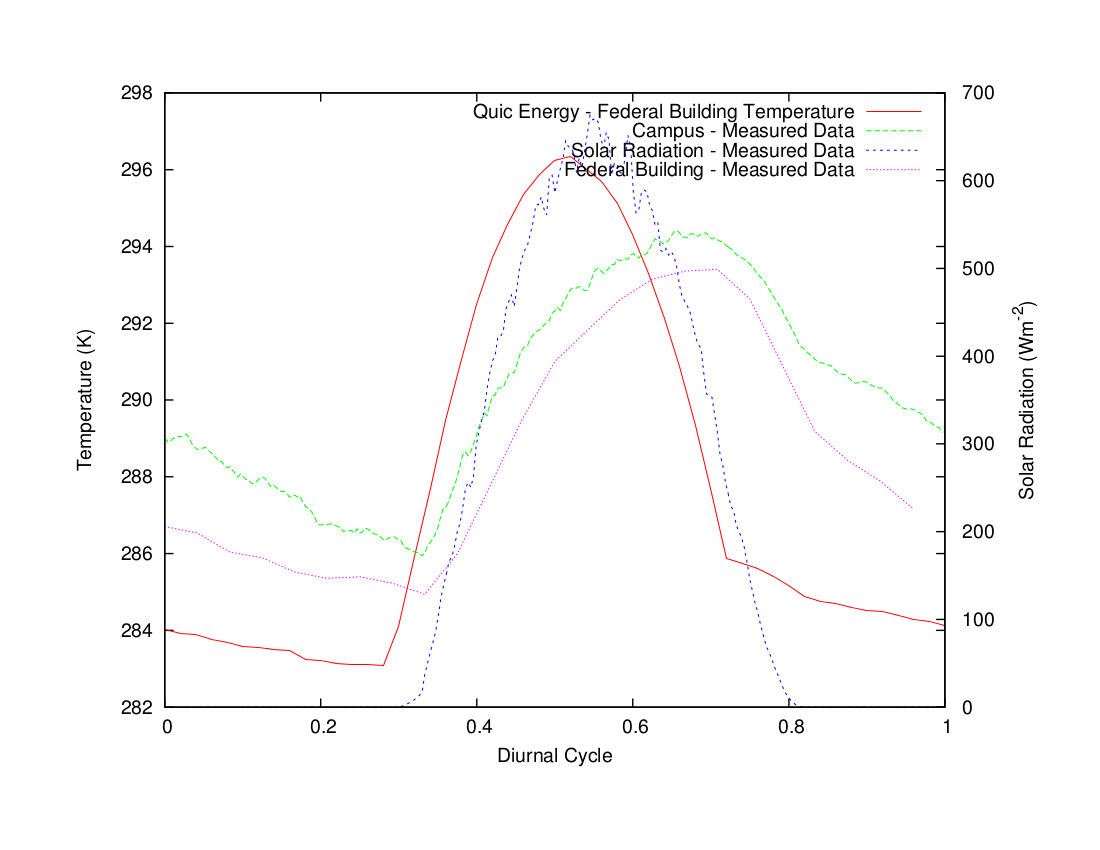
\includegraphics[width=0.8\linewidth]{images/goodData.png}
\caption{Good data.}
\label{fig:goodData}
\end{figure} 

We can reference the plot in Figure~\ref{fig:goodData}. Also, it's sometimes nice to include tables.

\begin{table}
\begin{center}
  \begin{tabular}{ | l | l | l | }
    \hline
    Variable & Condition 1 & Condition 2 \\ \hline
    \(arc\) & 1.796 & 0.304 \\ \hline 
    \(boo\) & 3.112 & 0.411 \\ \hline 
    \(gar\) & 4.344 & 0.629 \\ 
    \hline
  \end{tabular}
\end{center}
\caption{Illustrates the relationship between variables and the related experiment conditions.}
\label{tid:dataCond12}
\end{table}
